\chapter{Fassolakia}
\label{ch:fassolakia}
\index{meal}
\index{green beans}
\index{tomato}

\marginnote{
    \textbf{Makes 8+ servings} \\
    Prep time: 15-20 minutes \\
    Cook time: 1-2 hours \\
    \vspace*{\baselineskip}

    1 large onion, chopped \\
    1 bag green beans \\
    1 can tomato sauce, Hunt's (213ml) \\
    1/2 cup parsley, chopped \\
    Salt \\
    Oil \\
    3-5 red potatoes, peeled and quartered (keep in cold water) 
}

\textit{Green beans with potatoes}

Family member: Mom

% \begin{figure}
%   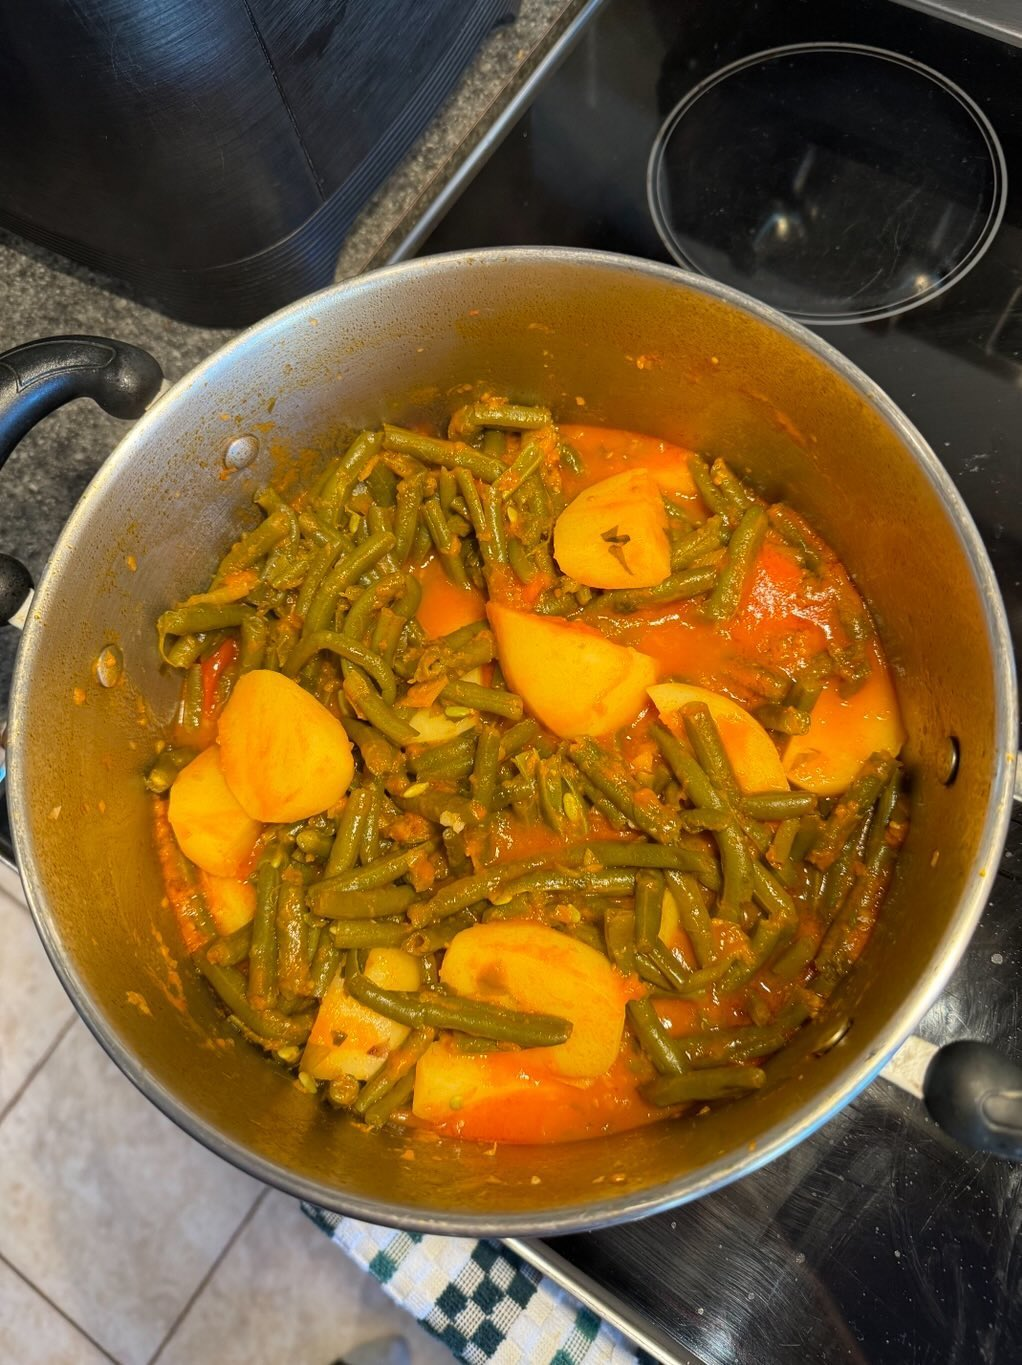
\includegraphics[width=60mm]{monanteras/images/Green beans 1.jpg}
%   \caption{Fassolakia}
% \end{figure}

\marginalfigure{monanteras/images/Green beans 1.jpg}{Fassolakia}{fig:fassolakia}

\begin{enumerate}
    \item Wash green beans and remove both edges.
    \item Drizzle a little of oil in a large pot, add onion once heated. Cook on medium heat.
    \item When the onion is translucent, add the green beans and mix. Add the tomato sauce, stir and add water until all the beans are covered.
    \item Add chopped parsley, salt and mix.
    \item Bring to a boil and keep it simmering uncovered until the beans are softened, about 45 minutes.
    \item Add the potatoes and keep cooking. Add a little water if necessary to cover potatoes.
    \item When you can poke the potatoes with a knife and the sauce has reduced, remove the pot from the heat and cover. Let cool for about 1 hour before eating.
\end{enumerate}

Eat with a large piece of feta and village bread!

